\section{Technical Approach}
\label{sec:techapp}

The system consists of a camera that points towards the user. The user should be wholly within the camera's frame of view. ~\figref{fig:camview} portrays the camera's point of view. The software of the system has three primary stages and they occur in the following order: detection, tracking and control. The system flow is outlined below:

%=================================================================
\begin{figure}[htbp]
	\begin{center}
		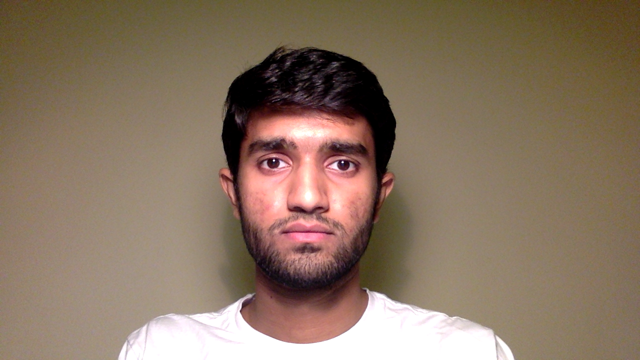
\includegraphics[width=\textwidth]{pics/cameraView.png}
	\end{center}%
	\caption{Camera's Frame of View}
	\label{fig:camview}
\end{figure}%
%=================================================================

\begin{enumerate}
	\item The user first selects their face by drawing a rectangular box around it. The selected face is used as template whenever the face needs to be detected.
	\item Once the face is detected, the system extracts features from the detected region.
	\item The extracted features are then tracked as the user moves their head around in order to control the mouse pointer.
	\item The movement of the user's head is translated into movement of the mouse pointer on the computer.
	\item If the tracked features are lost at any point during the tracking phase, the face is detected again using the template that was provided by the user in (1).
\end{enumerate}

The following subsections describe the ways in detection, tracking and pointer-control are performed. 

\subsection{Face Detection}

The system performs detection using template matching of Histogram Of Gradients (HOG). To perform detection, the HOG of the user's face (initially selected by the user) is matched against the HOG of the image that corresponds to the camera's view. The HOGs of an image is computed by dividing the image into $8\times8$ disjoint block of pixels. The orientation of each of these blocks is binned into 9 equal spaced bins between $-pi/2$ and $pi/2$. Hence, an image with height, $H$, and width, $W$, will have a HOG represented by a three-dimensional array with the dimensions of $H/8 \times W/8 \times 9$. Cross-correlation is used to compare the HOGs of two images. After performing non-maxima suppression, the $8 \times 8$ block with the largest cross-correlation measure is considered to be the center of the detected face. ~\figref{fig:detection} depicts the HOG of the face region selected by the user and the resulting detection on the camera's frame of view.

%=================================================================
\begin{figure}[htbp]
	\centering
	%-------------------------------------------------------------------------------------------
	\begin{minipage}[t]{0.24\textwidth}\centering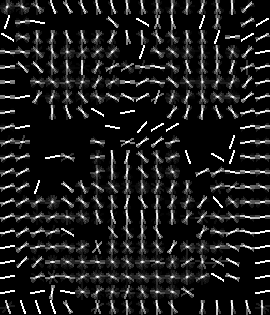
\includegraphics[width=\textwidth]{pics/faceHOG.png}\par(a) Face's HOG \end{minipage}
	\begin{minipage}[t]{0.74\textwidth}\centering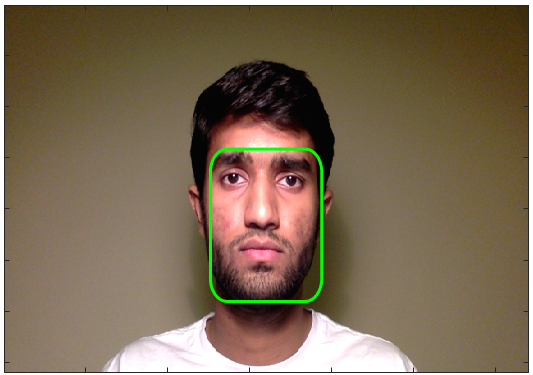
\includegraphics[width=\textwidth]{pics/detectedFace.png}\par(b) Detected Face \end{minipage}
	%-------------------------------------------------------------------------------------------
	\caption{Face detection using HOG}
	\label{fig:detection}
\end{figure}
%=================================================================

\subsection{Face Tracking}

Once the face is detected, the initial features in the detected region are extracted using the minimum eigenvalue algorithm ~\cite{shi1994good} (see Section ~\ref{sec:discussion} for initial approaches used).~\figref{fig:features} depicts the features selected by this algorithm.

The feature points are then tracked using the Kanade-Lucas-Tomasi (KLT) algorithm ~\cite{tomasi1991detection}. In order to make the tracking robust, the threshold for the bidirectional error of the KLT is set to 3 pixels. To implement the feature extraction and the tracking algorithms, I used the MATLAB functions and objects, \texttt{detectMinEigenFeatures}~\cite{mineigen} and \texttt{PointTracker}~\cite{pointtracker} from the Computer Vision System Toolbox ~\cite{cvtoolbox}. If the lighting conditions are not constant or if the head movements are too fast, a significant portion of the feature trackers are lost. Hence, when less than 10 feature points remain, the system notifies the user about the loss of tracking, asks the user to stay still and re-detects the face of the user using the HOG of the template specified by the user. ~\figref{fig:tracking} shows the tracking of the same features in different head poses. The red star in the figure demarcates the head-position (the mean position of all features)

%=================================================================
\begin{figure}[htbp]
	\begin{center}
		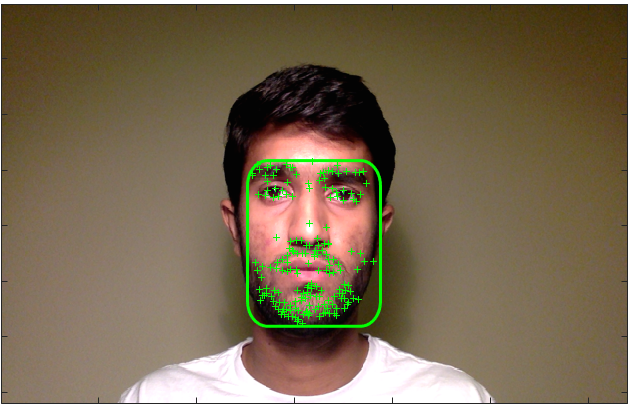
\includegraphics[width=0.9\textwidth]{pics/detectedFeatures.png}
	\end{center}%
	\caption{Features detected by the minimum eigenvalue algorithm}
	\label{fig:features}
\end{figure}%
%=================================================================


%=================================================================
\begin{figure*}[htbp]
	%\vspace{-20pt}
	\centering
	%-----------------------------------------------------------------------------------------
	\begin{minipage}[t]{0.49\textwidth}\centering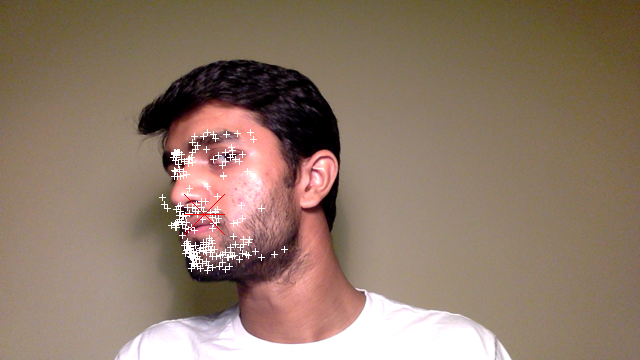
\includegraphics[width=\textwidth]{pics/leftTracking.png}\par(a) Facing Left  \end{minipage}
	\begin{minipage}[t]{0.49\textwidth}\centering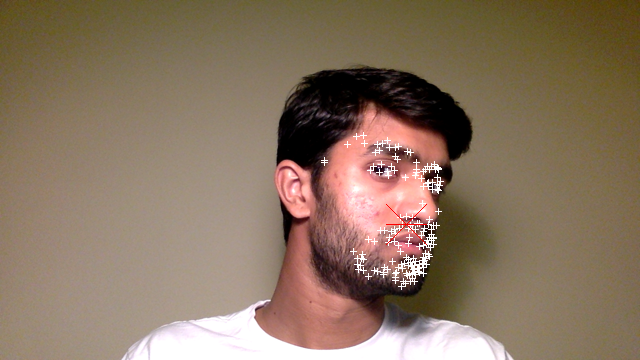
\includegraphics[width=\textwidth]{pics/rightTracking.png}\par(b) Facing Right \end{minipage}
	\begin{minipage}[t]{0.49\textwidth}\centering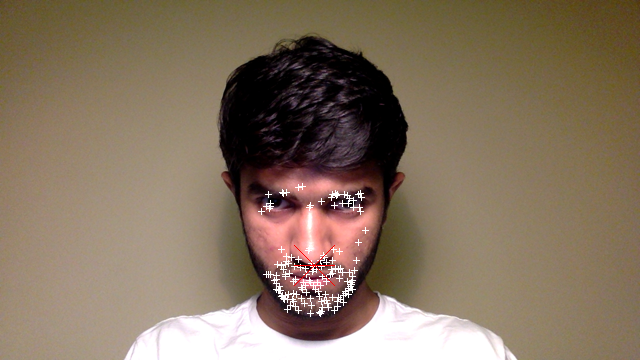
\includegraphics[width=\linewidth]{pics/downTracking.png}\par(c) Facing Down \end{minipage}
	\begin{minipage}[t]{0.49\textwidth}\centering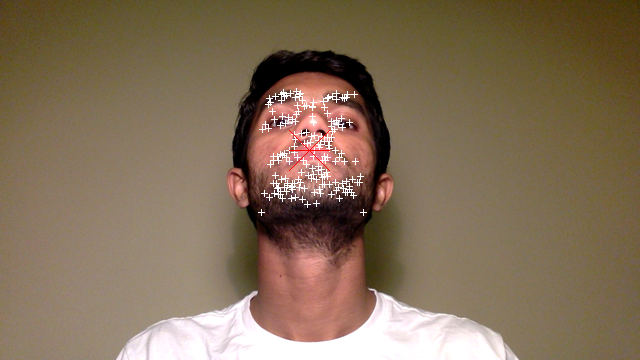
\includegraphics[width=\linewidth]{pics/upTracking.png}\par(d)  Facing Up \end{minipage}
	%-----------------------------------------------------------------------------------------
	\caption{Feature tracking in different head poses.}
	\label{fig:tracking}
\end{figure*}
%=================================================================



\subsection{Pointer Control}

To control the mouse pointer according to the head movements, I use a linear Rate Control approach ~\cite{kjeldsen2006improvements}. In a Rate Control approach, the movement of the pointer depends only on the succeeding motions of the head and doesn't consider any absolute reference position/frame.

When the face has been detected and the tracker has been initialized, I se the mouse pointer to the center of the screen. In every frame, I compute the mean of the x-coordinates of all the feature points and the mean of the y-coordinates of all the feature points being tracked and use the resulting means to demarcate the "head-position." I compute the displacement, $x$ of this position w.r.t the same in the previous frame. I apply $Ax$, a scaled version of this displacement to determine the next coordinates of the mouse pointer. Empirically, a value of 15 for $A$ worked reasonably well.